\documentclass[11pt]{article}

\usepackage[a4paper,margin=2.5cm]{geometry}
\usepackage{graphicx}
\usepackage{amsmath,amssymb}
\usepackage{booktabs}
\usepackage{hyperref}
\usepackage{xcolor}
\usepackage{caption}
\usepackage{float}

\hypersetup{
  colorlinks=true,
  linkcolor=blue,
  urlcolor=blue,
}

\title{Trustworthy Machine Learning -- Spring 2026\\
       Homework Assignment 1}
\author{ID: 205455207}
\date{}

\begin{document}
\maketitle

\section*{Question \#1 -- White-box vs.\ query-based black-box attack}

\paragraph{1. Benign accuracy.}
After implementing \texttt{utils.compute\_accuracy}, the (benign) accuracy of
\texttt{simple-cnn-0} on the supplied 200-image test set is
\[
\boxed{\mathrm{acc} = \texttt{0.8750}}.
\]

\paragraph{2. White-box PGD success rates.}
Running \texttt{main\_a.py} with our \texttt{PGDAttack} (\(\epsilon=8/255\),
\(\alpha=1/255\), 50 iterations, random initialisation, early stopping)
yields the following success rates against \texttt{simple-cnn-0}:
\begin{center}
\begin{tabular}{lc}
\toprule
Attack & Success rate \\
\midrule
Untargeted PGD (white-box) & \texttt{0.9850} \\
Targeted PGD (white-box)   & \texttt{0.9400} \\
\bottomrule
\end{tabular}
\end{center}
For targeted attacks, target labels are drawn at random with
\(t = (c_x + \mathrm{randint}(1,n_{\mathrm{classes}}))\bmod n_{\mathrm{classes}}\),
guaranteeing \(t\neq c_x\).

\paragraph{3. Black-box NES-PGD success rates.}
We implemented \texttt{NESBBoxPGDAttack} using antithetic sampling: at every
PGD iteration we draw \(k=200\) Gaussian noise tensors \(u_i\) and query the
model on \(x\pm\sigma u_i\) (so a total of \(2k=400\) queries per iteration
per active sample). The gradient is approximated as
\[
\widehat{\nabla_x \mathrm{loss}} \;=\;
   \frac{1}{2k\sigma}\sum_{i=1}^{k}\,\bigl[\mathrm{loss}(x+\sigma u_i)-\mathrm{loss}(x-\sigma u_i)\bigr]\, u_i .
\]
With momentum \(\mu\) the update used at iteration \(t\) is
\(g_t = \mu\, g_{t-1} + \widehat{\nabla_x\mathrm{loss}}_t\), and PGD takes the
sign of \(g_t\). Results (success rates and median number of model queries):
\begin{center}
\begin{tabular}{lcccc}
\toprule
& \multicolumn{2}{c}{Untargeted} & \multicolumn{2}{c}{Targeted}\\
\cmidrule(lr){2-3}\cmidrule(lr){4-5}
& success & median \#queries & success & median \#queries \\
\midrule
NES-PGD, \(\mu=0.0\) & \texttt{0.9250} & \texttt{3600} & \texttt{0.7500} & \texttt{7600} \\
NES-PGD, \(\mu=0.9\) & \texttt{0.9650} & \texttt{2400} & \texttt{0.8650} & \texttt{4000} \\
\bottomrule
\end{tabular}
\end{center}

\paragraph{Comparison with white-box.}
The black-box NES attack is markedly less query-efficient than white-box PGD,
which only needs one back-prop per iteration; the black-box attack also tends
to have slightly lower success rates (especially for targeted attacks), since
the NES gradient estimate is noisier than the true gradient. In our run the
white-box attack reaches \texttt{0.9850}/\texttt{0.9400}
(untargeted/targeted) while the best black-box configuration reaches
\texttt{0.9650}/\texttt{0.8650}.

\paragraph{Effect of momentum.}
Adding momentum \(\mu=0.9\) to the NES-PGD attack \emph{both raises the
success rate and reduces the number of model queries}: the success rate
climbs from \texttt{0.9250} to \texttt{0.9650} (untargeted, \(+4.0\) p.p.)
and from \texttt{0.7500} to \texttt{0.8650} (targeted, \(+11.5\) p.p.),
while the median number of queries drops from \texttt{3600} to \texttt{2400}
(untargeted) and from \texttt{7600} to \texttt{4000}
(targeted). Intuitively, the NES gradient estimator is a stochastic
finite-difference estimator -- each iteration produces a noisy estimate of
the same underlying gradient. Accumulating a fraction of the previous
gradient acts as an exponential moving average that suppresses estimation
noise and reinforces directions that have been consistently useful across
iterations, leading PGD to escape the eps-ball boundary along a more
informative direction in fewer iterations (each iteration costs the same
\(2k\) queries, so fewer iterations means fewer queries).

\begin{figure}[H]
\centering
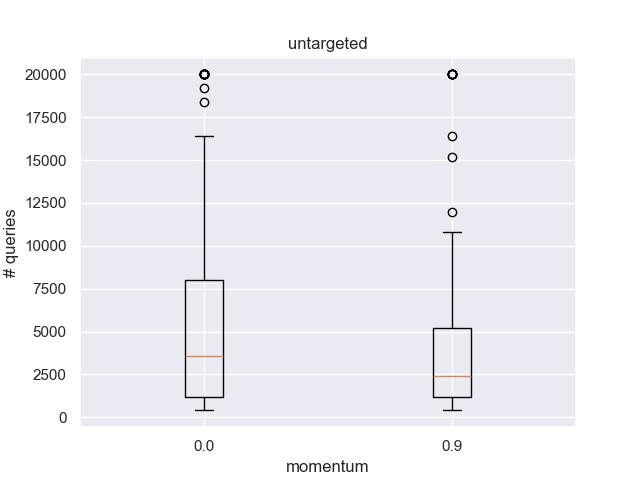
\includegraphics[width=0.48\textwidth]{bbox-n_queries_untargeted.jpg}
\hfill
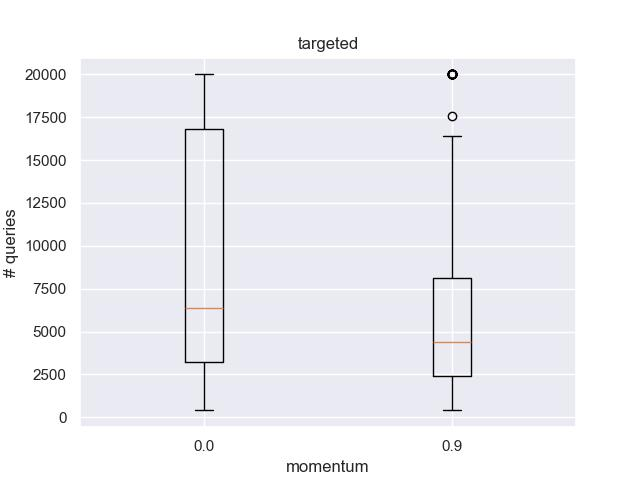
\includegraphics[width=0.48\textwidth]{bbox-n_queries_targeted.jpg}
\caption{Number of queries used by the NES-PGD black-box attack on
\texttt{simple-cnn-0}, with and without momentum, for untargeted (left) and
targeted (right) attacks. Distributions over the 200 images of the test set.}
\end{figure}


\section*{Question \#2 -- Transferability-based black-box attack}

\paragraph{Single-model transferability.}
Using our white-box PGDAttack against each of the three pre-trained CNNs,
we obtain the following matrices of success rates. The \((i,j)\) entry is
the rate at which adversarial examples crafted on the surrogate
\texttt{simple-cnn-}\(i\) (rows) succeed against the target
\texttt{simple-cnn-}\(j\) (columns).
The diagonal corresponds to white-box attacks; the off-diagonal entries
quantify transferability.

\textbf{Untargeted}:
\[
\begin{pmatrix}
\texttt{0.985} & \texttt{0.570} & \texttt{0.535} \\
\texttt{0.690} & \texttt{0.965} & \texttt{0.585} \\
\texttt{0.585} & \texttt{0.545} & \texttt{0.950}
\end{pmatrix}
\]

\textbf{Targeted}:
\[
\begin{pmatrix}
\texttt{0.945} & \texttt{0.315} & \texttt{0.265} \\
\texttt{0.410} & \texttt{0.865} & \texttt{0.285} \\
\texttt{0.360} & \texttt{0.275} & \texttt{0.845}
\end{pmatrix}
\]

\paragraph{Discussion.}
Untargeted PGD adversarial examples transfer reasonably well between these
three CNNs: off-diagonal success rates are in the range
\([\texttt{0.535},\,\texttt{0.690}]\), well above the
\(1{-}\mathrm{acc}\approx 0.13\) baseline of merely returning misclassified
images. In contrast, targeted attacks transfer significantly worse: the
off-diagonal entries are in the range
\([\texttt{0.265},\,\texttt{0.410}]\), as expected since
targeting a specific (wrong) class requires the surrogate's gradient to
align with the target model's gradient on a much narrower direction.

\paragraph{Ensemble attack.}
After implementing \texttt{PGDEnsembleAttack} (which descends the average
cross-entropy loss across the ensemble at every PGD step) we craft
adversarial examples against the ensemble \(\{\texttt{simple-cnn-1},
\texttt{simple-cnn-2}\}\) and evaluate them on \texttt{simple-cnn-0}:
\begin{center}
\begin{tabular}{lcc}
\toprule
Attack source & Untargeted SR on cnn-0 & Targeted SR on cnn-0 \\
\midrule
single surrogate cnn-1                   & \texttt{0.690} & \texttt{0.410} \\
single surrogate cnn-2                   & \texttt{0.585} & \texttt{0.360} \\
ensemble \{cnn-1, cnn-2\} (Liu et al.)   & \texttt{0.7400} & \texttt{0.5050} \\
\bottomrule
\end{tabular}
\end{center}
Both untargeted and targeted transferability \emph{improve} when attacking
the ensemble: the untargeted success rate on \texttt{simple-cnn-0} climbs
from \(\max(\texttt{0.690},\texttt{0.585})=\texttt{0.690}\)
to \texttt{0.7400} (an absolute boost of
\(\texttt{+5.0}\) percentage points), and the targeted success
rate climbs from \texttt{0.410} to \texttt{0.5050}
(\(\texttt{+9.5}\) p.p.). Intuitively, an adversarial example
crafted to fool \emph{multiple} surrogates simultaneously must exploit
features that are common to several models, and is therefore more likely to
exploit features shared with an unseen target as well; this shared, less
model-specific perturbation generalises better to the held-out model
\texttt{simple-cnn-0}, exactly as predicted by Liu et al.~\cite{liu2017}.


\section*{Question \#3 -- Bit-flip attacks}

We implement IEEE-754 single-precision (\texttt{float32}) bit conversion
helpers (\texttt{utils.binary} and \texttt{utils.float32}) and a random
bit-flip routine (\texttt{utils.random\_bit\_flip}). We then iterate over
the five layers of \texttt{simple-cnn-1} (\texttt{conv1}, \texttt{conv2},
\texttt{fc1}, \texttt{fc2}, \texttt{fc3}) and, for each layer, perform
\(\texttt{BF\_PER\_LAYER}=450\) bit flips: at each step we sample a random
weight and a random bit index in \(\{0,\dots,31\}\), flip the bit, measure
the relative accuracy drop
\[
\mathrm{RAD} \;=\; \frac{\mathrm{acc}_{o}-\mathrm{acc}_{bf}}{\mathrm{acc}_{o}},
\]
and restore the weight. The original (pre-flip) accuracy of
\texttt{simple-cnn-1} on the test set is
\(\mathrm{acc}_o = \texttt{0.8250}\). In total \(450\times 5 = 2250\)
bit-flips were performed.

\begin{enumerate}
\item \textbf{Maximum RAD:} \(\boxed{\texttt{0.7273}}\).
\item \textbf{Fraction of bits with RAD \(>15\%\):} \(\boxed{\texttt{2.62\%}}\)
of all 2250 flips.
\item \textbf{Per-bit median RAD.} The box-plot in
Figure~\ref{fig:bf-idx} summarises the RAD distribution as a function of
the flipped bit index (big-endian: index 0 is the sign bit, indices 1--8
are the exponent, indices 9--31 are the mantissa).
The bit with the highest median RAD is index
\(\boxed{\texttt{1}}\), corresponding to the
\textbf{most-significant bit of the IEEE-754 exponent}.
\end{enumerate}

\paragraph{Why is the MSB of the exponent the most damaging?}
The IEEE-754 binary32 format encodes a value as
\(x = (-1)^{s}\,(1+m)\cdot 2^{e-127}\), where \(s\) is the sign bit,
\(e\in\{0,\dots,255\}\) is the (biased) exponent, and \(m\in[0,1)\) is the
mantissa. Trained neural-network weights are typically of magnitude
\(\ll 1\), so their unbiased exponent is negative and the biased exponent
\(e\) is comfortably below \(127\), meaning the MSB of \(e\) (i.e.\ the
\(2^{7}=128\) bit of the exponent field) is almost always 0. Flipping this
bit from 0 to 1 \emph{adds 128 to the exponent} and multiplies the weight
by \(2^{128}\approx 3.4\times 10^{38}\) -- typically the value becomes
\texttt{inf} or saturates downstream activations to NaN/Inf, devastating
the model's prediction. By contrast, flipping a mantissa bit changes the
weight by at most a factor of \(\sim\!2\) (and usually far less) and
flipping the sign bit just negates a small number; both have a much milder
effect on accuracy.

\begin{figure}[H]
\centering
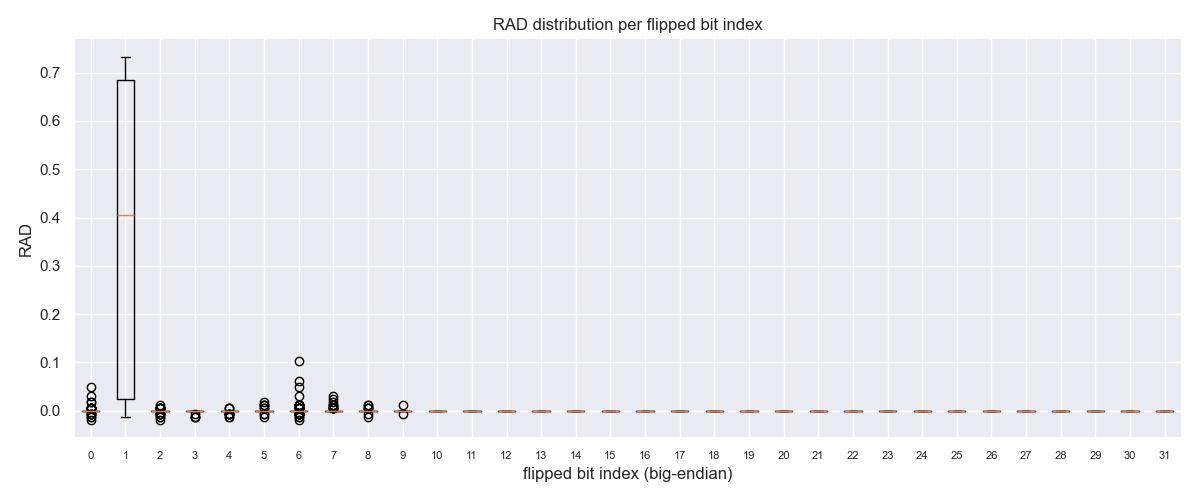
\includegraphics[width=\textwidth]{bf_idx-vs-RAD.jpg}
\caption{Box-plot of RAD distribution per flipped bit index (big-endian
IEEE-754, bit~0 = sign, bits~1--8 = exponent, bits~9--31 = mantissa)
on \texttt{simple-cnn-1}. Bit~\texttt{1} (the MSB of the
exponent) has the highest median RAD.}
\label{fig:bf-idx}
\end{figure}

\begin{thebibliography}{9}
\bibitem{hong2019} S.~Hong, P.~Frigo, Y.~Kaya, C.~Giuffrida, and T.~Dumitras.
  \emph{Terminal brain damage: Exposing the graceless degradation in deep neural networks under hardware fault attacks.}
  Proc.\ USENIX Security, 2019.
\bibitem{ilyas2018} A.~Ilyas, L.~Engstrom, A.~Athalye, and J.~Lin.
  \emph{Black-box adversarial attacks with limited queries and information.}
  Proc.\ ICML, 2018.
\bibitem{liu2017} Y.~Liu, X.~Chen, C.~Liu, and D.~Song.
  \emph{Delving into transferable adversarial examples and black-box attacks.}
  Proc.\ ICLR, 2017.
\end{thebibliography}

\end{document}
